\documentclass[10pt,serif]{beamer}
\mode<presentation>
{
	%\usetheme{Pittsburgh}
	\usetheme[style=plain,sidebar=false]{uu}
	\setbeamertemplate{frametitle}[default][center]
	% or ...
% \usebeamerfont[serif]{Times}
	\setbeamercovered{transparent}
	% or whatever (possibly just delete it)
}
\usepackage{algpseudocode}
\usepackage[boxed]{algorithm}
\usepackage{algorithmicx}

\usepackage[english]{babel}
\usepackage{tikz}
\usepackage{subfigure}
\usepackage[absolute,overlay]{textpos}
\usetikzlibrary{chains}
\usetikzlibrary{shapes,arrows}
\newcommand {\argmin} {\mathop{\mathrm{argmin}}\limits}
\newcommand{\R}{\mathbb{R}}
\setbeamertemplate{itemize subitem}{$\diamond$}
\setlength{\parskip}{6pt} %%distanza fra i paragrafi
%adjust the TPHorizModule and TPHorizModule units to the displayed mm %grid 
\TPGrid{210}{297} 
\tikzstyle{myred}=[red!90,opacity=.8]
\tikzstyle{myblue}=[blue!60!cyan,opacity=.9]
\tikzstyle{mypurple}=[purple!80!blue,opacity=.9]
\tikzstyle{myblack}=[gray!10!black,opacity=.9]
\tikzstyle{mygreen}=[yellow!60!cyan,opacity=.9]
\tikzstyle{myarrow}=[line width=1.3pt,>=latex,->]
\tikzstyle{vertex} = [fill,shape=circle,node distance=100pt,minimum size=0.2cm,inner sep = 0pt]

%\usepackage{Times}
%\usepackage[T1]{fontenc}
% Or whatever. Note that the encoding and the font should match. If T1
% does not look nice, try deleting the line with the fontenc.


\title % (optional, use only with long paper titles)
{Iterative sparse matrix partitioning}

\subtitle{\emph{Supervisor:} Prof. dr. Rob H. Bisseling}

\author % (optional, use only with lots of authors)
{Davide Taviani}
% - Use the \inst{?} command only if the authors have different
%   affiliation.

\date{October 7th, 2013}

\subject{Matrix partitioning}
% This is only inserted into the PDF information catalog. Can be left
% out.


% If you have a file called "university-logo-filename.xxx", where xxx
% is a graphic format that can be processed by latex or pdflatex,
% resp., then you can add a logo as follows:

%\pgfdeclareimage[height=1.2cm]{university-logo}{UULogo.png}
%\logo{\pgfuseimage{university-logo}}

% If you wish to uncover everything in a step-wise fashion, uncomment
% the following command:

%\beamerdefaultoverlayspecification{<+->}

%\AtBeginSection[]
%{
%	\begin{frame}{Table of Contents}
%		\tableofcontents%[currentsection,currentsubsection]
% \end{frame}
%}
			

\begin{document}

\begin{frame}
	\titlepage
\end{frame}

\section{Introduction}

\subsection{Parallel sparse matrix-vector multiplication}
\begin{frame}{Parallel sparse matrix-vector multiplication}

At the core of many iterative solvers (e.g. conjugate gradient method) lies a simple operation: \textbf{sparse matrix-vector multiplication}.

\vspace{0.5cm}

Given:
\begin{itemize}
	\item $m \times n$ sparse matrix $A$ ($N$ nonzeros, $N \ll mn$)
	\item $n \times 1$ vector $\vec{v}$
\end{itemize}

we want to compute

	$$\vec{u}=A\vec{v}$$

\end{frame}

\begin{frame}{Parallel sparse matrix-vector multiplication}

	Usually $A$ is fairly large and a lot of computations are required:
	\begin{itemize}
		\item $\mathcal{O}(mn)$ following the definition of matrix-vector multiplication;
		\item $\mathcal{O}(N)$ only considering the nonzero elements. 
	\end{itemize}
	
	We split the computations among $p$ processors to improve speed.

	We make a \textbf{partition} of the set of the nonzeros of $A$, obtaining $p$ disjoint sets $A_0,\dots,A_{p-1}$.

	Furthermore, also the input vector $\vec{v}$ and the final output $\vec{u}$ can be divided among those $p$ processors (their distribution might not necessarily be the same).

\end{frame}

\subsection{Matrix partitioning}

\begin{frame}{Matrix partitioning}

	Example of a partition of a $9 \times 9$ matrix with 18 nonzeros, with $p=2$.

	\begin{figure}[h]
	\centering
	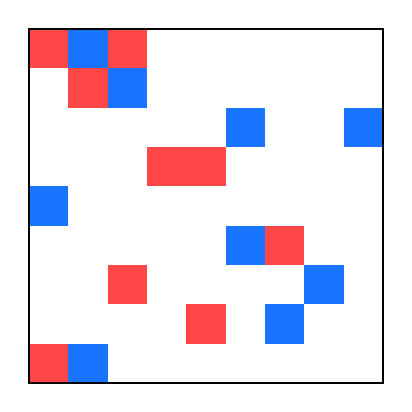
\begin{tikzpicture}[scale=0.5]
		\foreach \x / \y in {1/1,1/3,2/2,4/5,4/4,7/3,8/5,6/7,9/1} { \fill[red!90,opacity=.8] ({\y-1},{-\x+1}) rectangle +(1,-1);}
		\foreach \x / \y in {1/2,2/3,3/6,3/9,6/6,5/1,7/8,8/7,9/2} { \fill[blue!60!cyan,opacity=.9] ({\y-1},{-\x+1}) rectangle +(1,-1);}
%		\draw[semithick] (0,-9) grid (9,0);
		\draw[thick] (0,-9) rectangle (9,0);
	\end{tikzpicture}
\end{figure}


\end{frame}
\begin{frame}{Matrix partitioning}

Local view of the matrix for every processor:

	\begin{figure}[h]
	\centering
	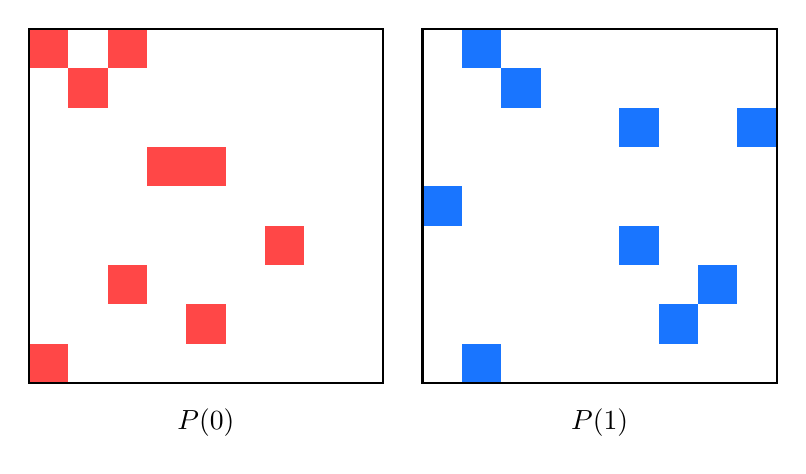
\begin{tikzpicture}[scale=0.5]
		\foreach \x / \y in {1/1,1/3,2/2,4/5,4/4,7/3,8/5,6/7,9/1} { \fill[red!90,opacity=.8] ({-10+\y-1},{-\x+1}) rectangle +(1,-1);}
		\foreach \x / \y in {1/2,2/3,3/6,3/9,6/6,5/1,7/8,8/7,9/2} { \fill[blue!60!cyan,opacity=.9] ({\y-1},{-\x+1}) rectangle +(1,-1);}
		\draw[thick] (-10,-9) rectangle (-1,0);
		\draw[thick] (0,-9) rectangle (9,0);
		\node at (-5.5,-10) {$P(0)$};
		\node at (4.5,-10) {$P(1)$};
	\end{tikzpicture}
\end{figure}


\end{frame}


\begin{frame}{Parallel matrix-vector multiplication algorithm}
		Parallel sparse matrix-vector multiplication is made (essentially) by 4 phases:

	\begin{enumerate}[I)]\itemsep=0.4cm
			\item \textbf{fan-out}%: each processor receives the required elements of $\vec{v}$ from the others (according to its distribution)
			\item \textbf{local multiplication}%: where the actual computation is performed
			\item \textbf{fan-in}%: where each processor sends his contributions to the other processors according to the distribution of $\vec{u}$
			\item \textbf{sum of all the contributions}
		\end{enumerate}
\end{frame}

\begin{frame}{Parallel matrix-vector multiplication algorithm}
	\begin{textblock}{170}(20,50)
		\only<1>{$A$ is partitioned along with $u$ and $v$}
		\only<2>{\textbf{Fan-out}:	each processor receives the required elements of $\vec{v}$ from the others (according to its distribution)}

		\only<3>{\textbf{Local multiplication}: where the actual computation is performed}

		\only<4>{\textbf{Fan-in}: where each processor sends his contributions to the other processors according to the distribution of $\vec{u}$}

\end{textblock}

	\begin{textblock}{100}(45,80)
	
	\begin{figure}[h]
	\centering
	\begin{tikzpicture}[scale=0.4]
		\foreach \x / \y in {1/1,1/3,2/2,4/5,4/4,7/3,8/5,6/7,9/1} { \fill[red!90,opacity=.8] ({\y-1},{-\x+1}) rectangle +(1,-1);}
		\foreach \x / \y in {1/2,2/3,3/6,3/9,6/6,5/1,7/8,8/7,9/2} { \fill[blue!60!cyan,opacity=.9] ({\y-1},{-\x+1}) rectangle +(1,-1);}

%		\draw[semithick] (0,-9) grid (9,0);
		\draw[thick] (0,-9) rectangle (9,0);

		\foreach \x in {2,4,5,7} { \fill[red!90,opacity=.8] ({\x-1},4) rectangle +(1,-1);}
		\foreach \x in {1,3,6,8,9} { \fill[blue!60!cyan,opacity=.9] ({\x-1},4) rectangle +(1,-1);}

\only<2>{
	\foreach \x in {1,3} { \draw[line width=2pt,blue!60!cyan,opacity=.9,->,>=latex] ({\x-0.5},2.8) -- ({\x-0.5},0.2);}
		\foreach \x in {2,7} { \draw[line width=2pt,red!90,opacity=.8,->,>=latex] ({\x-0.5},2.8) -- ({\x-0.5},0.2);}
	}
%	\draw[->,very thick,>=latex] ({7-0.5},1.8) -- ({7-0.5},{-7+0.2});
%		\draw[semithick] (0,3) grid (9,4);
		\draw[thick] (0,3) rectangle (9,4);

		\foreach \x in {2,4,6,7,9} { \fill[red!90,opacity=.8] (-4,{-\x+1}) rectangle +(1,-1);}
		\foreach \x in {1,3,5,8} { \fill[blue!60!cyan,opacity=.9] (-4,{-\x+1}) rectangle +(1,-1);}

\only<4>{		\foreach \x in {1,8} { \draw[line width=2pt,red!90,opacity=.8,->,>=latex] (-0.2,{-\x+0.5}) -- (-2.8,{-\x+0.5});}
		\foreach \x in {2,6,7,9} { \draw[line width=2pt,blue!60!cyan,opacity=.9,->,>=latex] (-0.2,{-\x+0.5}) -- (-2.8,{-\x+0.5});}
	}
%		\draw[semithick] (-4,-9) grid (-3,0);
		\draw[thick] (-4,-9) rectangle (-3,0);
		\node at (-3.5,-9.5) {$u$};
		\node at (9.5,3.5) {$v$};
		\node at (9.5,-9.5) {$A$};
	\end{tikzpicture}
\end{figure}
\end{textblock}
\end{frame}
\begin{frame}{Matrix partitioning}

	To optimize this process:

	\begin{itemize}
		\item I and III involve communication: it has to be \textbf{minimized}
		\item II is a computation step: we need \textbf{balance} in the size of the partitions
	\end{itemize}

	\textbf{Optimization problem}: partition the nonzeros such that the balance constraint is satisfied and the communication volume is minimized.

\end{frame}

\begin{frame}{Matrix partitioning}
	As a last example, a $6 \times 6$ ``checkerboard'' matrix:

	\begin{figure}[h]
	\centering
	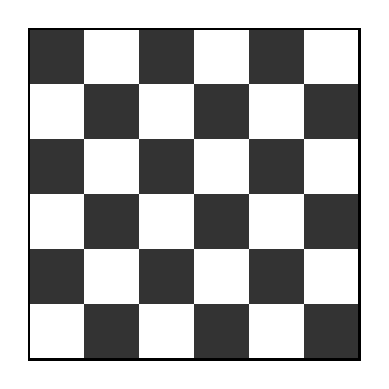
\begin{tikzpicture}[scale=0.7]
		\draw[thick] (0,0) rectangle (6,-6);
		\foreach \row in {0,1, ..., 5} {
			\foreach \column in {0, ..., 2} {
				\fill[opacity=.8] ({2*\column + mod(\row,2)}, -\row) rectangle +(1,-1);
			}
		};
%		\draw[semithick] (0,-6) grid (6,0);
	\end{tikzpicture}
\end{figure}

\end{frame}

\begin{frame}{Matrix partitioning}

	Two different partitionings result in extremely different communication volumes.

\begin{figure}[h]
	\centering
	\subfigure[Rows and columns are not split, therefore there is no need for communication.]{
		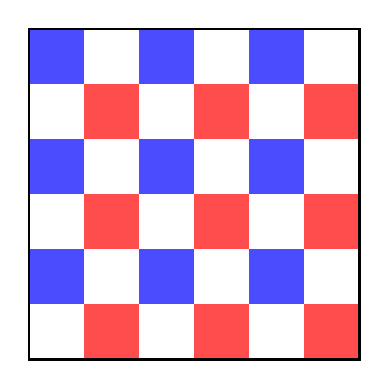
\begin{tikzpicture}[scale=0.7]
			\foreach \row in {0,2,4} {
				\foreach \column in {0, ..., 2} {
					\fill[opacity=.7,blue] ({2*\column + mod(\row,2)}, -\row) rectangle +(1,-1);
				}
			};
			\foreach \row in {1,3,5} {
				\foreach \column in {0, ..., 2} {
					\fill[opacity=.7,red] ({2*\column + mod(\row,2)}, -\row) rectangle +(1,-1);
				}
			};
%			\draw[semithick] (0,-6) grid (6,0);
			\draw[thick] (0,0) rectangle (6,-6);
		\end{tikzpicture} \label{fig:checkered_a}
	}\hspace{1cm}
	\subfigure[Every row and column is split and causes communication during fan-in and fan-out.]{
		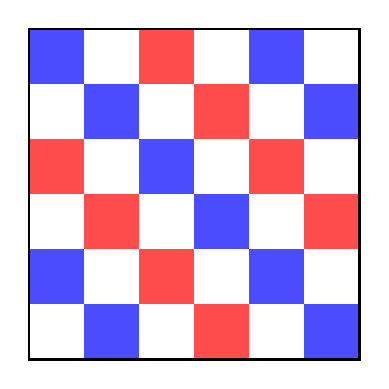
\begin{tikzpicture}[scale=0.7]
			\foreach \index in {0,1, ..., 5} {\fill[opacity=.7,blue] (\index, -\index) rectangle +(1,-1);};
			\foreach \index in {0,1, ..., 3} {\fill[opacity=.7,red] (2+\index, -\index) rectangle +(1,-1);};
			\foreach \index in {0,1, ..., 3} {\fill[opacity=.7,red] (\index, -2-\index) rectangle +(1,-1);};
			\foreach \index in {0,1} {\fill[opacity=.7,blue] (\index, -4-\index) rectangle +(1,-1);};
			\foreach \index in {0,1} {\fill[opacity=.7,blue] (4+\index, -\index) rectangle +(1,-1);};
%			\draw[semithick] (0,-6) grid (6,0);
			\draw[thick] (0,0) rectangle (6,-6);
		\end{tikzpicture} \label{fig:checkered_b}
	}
\end{figure}

\end{frame}

\subsection{Hypergraph partitioning}

\begin{frame}{Hypergraph partitioning}

The matrix partitioning can be viewed from the graph theory point of view:

\begin{itemize}
	\item Data represented as \emph{vertices}
	\item Connections represented as \emph{edges}
\end{itemize}

Further iteration: exact modeling of the matrix partitioning problem through \textbf{hypergraph partitioning}.
\end{frame}

\begin{frame}{Hypergraph partitioning}

	Hypergraph: a graph in which a \emph{hyperedge} can connect more than two \emph{vertices} (i.e. a subset of the vertex set $V$)

	\begin{figure}[h]
	\centering
\tikzstyle{vertex} = [fill,shape=circle,node distance=55pt]
\tikzstyle{edge} = [fill,opacity=.5,fill opacity=.5,line cap=round, line join=round, line width=50pt]
\tikzstyle{elabel} =  [fill,shape=circle,node distance=35pt]

\pgfdeclarelayer{background}
\pgfsetlayers{background,main}

\begin{tikzpicture}[scale=0.7,font=\small]
\node[vertex,label=above:\(v_1\)] (v1) {};
\node[vertex,right of=v1,label=above:\(v_2\)] (v2) {};
\node[vertex,below of=v1,label=above:\(v_4\)] (v4) {};
\node[vertex,right of=v4,label=above:\(v_5\)] (v5) {};
\node[vertex,left of=v4,label=above:\(v_3\)] (v3) {};
\node[vertex,below of=v4,label=above:\(v_7\)] (v7) {};
\node[vertex,left of=v7,label=above:\(v_6\)] (v6) {};

\begin{pgfonlayer}{background}
\draw[edge,color=blue] (v1) -- (v3) -- (v4) -- (v1);
\begin{scope}[transparency group,opacity=.5]
\draw[edge,opacity=1,color=green] (v4) -- (v7);
\end{scope}
\draw[edge,color=red] (v5) -- (v7);
\draw[edge,color=yellow] (v2) -- (v2);
\end{pgfonlayer}

\node[elabel,color=blue,label=right:{$e_1=\{v_1,v_3,v_4\}$}]  (e1) at (7,0) {};
\node[elabel,below of=e1,color=green,label=right:{$e_2=\{v_4,v_7 \}$}]  (e2) {};
\node[elabel,below of=e2,color=red,label=right:{$e_3=\left\{ v_5,v_7 \right\}$}]  (e3) {};
\node[elabel,below of=e3,color=yellow,label=right:{$e_4=\left\{ v_2 \right\}$}]  (e4) {};
\end{tikzpicture}
\end{figure}

\end{frame}

\begin{frame}{Hypergraph partitioning}

A partition of a hypergraph is simply the partition of the set of vertices $V$ into $V_0,\dots,V_{p-1}$.

A hyperedge $e = \{v_{e_1},\dots,v_{e_k}\}$ is \textbf{cut} if two of its vertices belong to different sets of the partition.
\end{frame}

\begin{frame}{Hypergraph partitioning}

	There are several models to translate the matrix partitioning to hypergraph partitioning:

	\begin{itemize}
		\item 1-dimensional
		\begin{itemize}\itemsep=0.3cm
				\item\textbf{row-net}: each column of $A$ is a vertex in the hypergraph, each row a hyperedge. If $a_{ij} \neq 0$, then column $A_i$ is placed in the hyperedge $j$.
				\item \textbf{column-net}: identical to the previous one, with the roles of columns and rows exchanged
			\end{itemize}
			\vspace{0.5cm}
As hypergraph partitioning consists in assignment of the vertices, columns/rows are uncut. Advantage of eliminating completely one source of communication, but being 1-dimensional is often a too strong restriction.
\end{itemize}
\end{frame}

\begin{frame}{Hypergraph partitioning}
	\begin{itemize}
		\item 2-dimensional (each nonzero independent)
			\begin{itemize}
					\vspace{0.2cm}
				\item \textbf{fine grain}: nonzeros of $A$ are vertices, rows and columns are hyperedges. The nonzero $a_{ij}$ is placed in the hyperedges $i$ and $j$

					\vspace{0.2cm}

				A lot of freedom in partitioning (each nonzero can be assigned individually), but the size of the hypergraph ($N$ vertices) is often too large.

					\vspace{0.2cm}
				\item \textbf{medium grain}: middle ground between 1-dimensional models and fine-grain

					\vspace{0.2cm}

					Middle ground between 1-dimensional models and fine grain: good compromise between the size of the hypergraph and freedom during the partitioning.

			\end{itemize}
	\end{itemize}

\end{frame}

\subsection{The medium-grain method}

\begin{frame}{Medium grain}

	(Daniel M. Pelt and Rob Bisseling, 2013, to appear)

	\begin{figure}[h]
	\centering
	\begin{tikzpicture}[scale=0.2]%,font=\large]
\only<1>{		\foreach \x / \y in {1/1,1/3,2/2,4/5,4/4,3/11,4/9,6/7,1/10,2/7} { \fill[myblack] ({\y-1},{-\x+1}) rectangle +(1,-1);}
		\foreach \x / \y in {1/2,2/3,3/6,3/9,6/6,5/1,5/12,6/10,2/11,2/8} { \fill[myblack] ({\y-1},{-\x+1}) rectangle +(1,-1);}
		\draw[thick] (0,-6) rectangle (12,0);
		\node at (6,-7) {$A$};
	}
	\only<2->{	
		\foreach \x / \y in {1/1,1/3,2/2,4/5,4/4,3/11,4/9,6/7,1/10,2/7} { \fill[purple!90,opacity=.8] ({\y-1},{-\x+1}) rectangle +(1,-1);}
		\foreach \x / \y in {1/2,2/3,3/6,3/9,6/6,5/1,5/12,6/10,2/11,2/8} { \fill[yellow!60!cyan,opacity=.9] ({\y-1},{-\x+1}) rectangle +(1,-1);}
		\draw[thick] (0,-6) rectangle (12,0);
		\node at (6,-7) {$A$};
	}
		\visible<2->{
		\foreach \x / \y in {1/1,1/3,2/2,4/5,4/4,3/11,4/9,6/7,1/10,2/7}{ \fill[purple!90,opacity=.8] ({18+\y-1},{-6-\x+1}) rectangle +(1,-1);}
		\node at (24,-13) {$A_c$};
		\draw[thick] (18,{-6-6}) rectangle ({18+12},-6);

		\foreach \x / \y in  {1/2,2/3,3/6,3/9,6/6,5/1,5/12,6/10,2/11,2/8} { \fill[yellow!60!cyan,opacity=.9] ({18+\y-1},{6-\x+1}) rectangle +(1,-1);}
		\node at (24,-1) {$A_r$};
		\draw[thick] (18,{-6+6}) rectangle ({18+12},6);
		\draw[line width=1.3pt,>=latex,->] (13,-3) -- (17,-9);
		\draw[line width=1.3pt,>=latex,->] (13,-3) -- (17,3);
	}
\visible<3->{
	\foreach \x / \y in {1/1,1/3,2/2,4/5,4/4,3/11,4/9,6/7,1/10,2/7}{ \fill[purple!90,opacity=.8] ({36+\y-1},{-6-\x+1}) rectangle +(1,-1);}
	\foreach \x / \y in  {1/2,2/3,3/6,3/9,6/6,5/1,5/12,6/10,2/11,2/8} { \fill[yellow!60!cyan,opacity=.9] ({48+\x-1},{6-\y+1}) rectangle +(1,-1);}
	\draw[line width=1.3pt,>=latex,->] (31,-9) -- (35,-4);
		\draw[line width=1.3pt,>=latex,->] (31,3) -- (35,-2);


		\foreach \x in {1,2,3,9,10,11} { \fill[gray!10!black,opacity=.9] ({36+\x-1},{6-\x+1}) rectangle +(1,-1);}
		\foreach \x in {1,2,3,6} { \fill[gray!10!black,opacity=.9] ({48+\x-1},{-6-\x+1}) rectangle +(1,-1);}

		\draw[thick] (36,-12) rectangle (54,6);
		\draw[ultra thick] (48,-12) -- (48,6);
		\draw[ultra thick] (36,-6) -- (54,-6);

		\node at (45,-13) {$B$};
	}
		
	\end{tikzpicture}
\end{figure}

\vspace{-0.4cm}

\begin{itemize}

	\visible<2->{\item Initial split of $A$ into $A^c$ and $A^r$}
	\visible<3->{	\item Construction of the $(m+n)\times (m+n)$ matrix $B$ (with dummy diagonal elements)}
	\end{itemize}

\end{frame}


\begin{frame}{Medium grain}

\begin{figure}[h]
	\centering
%	\includegraphics{img/mg-1}
	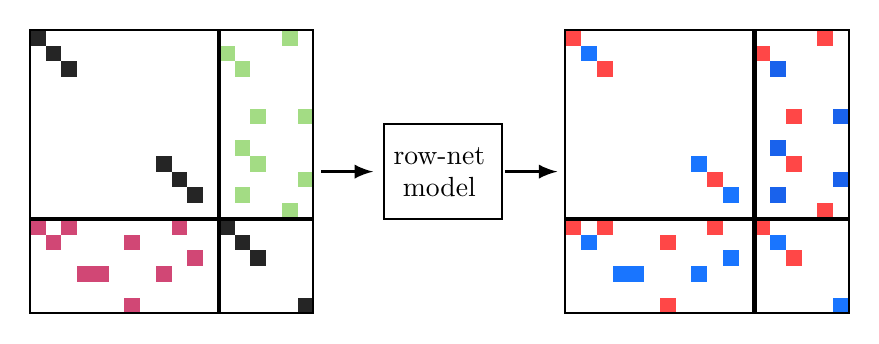
\begin{tikzpicture}[scale=0.2]

		\foreach \x / \y in {1/1,1/3,2/2,4/5,4/4,3/11,4/9,6/7,1/10,2/7}{ \fill[purple!90,opacity=.8] ({-34+\y-1},{-6-\x+1}) rectangle +(1,-1);}
		\foreach \x / \y in  {1/2,2/3,3/6,3/9,6/6,5/1,5/12,6/10,2/11,2/8} { \fill[yellow!60!cyan,opacity=.9] ({-22+\x-1},{6-\y+1}) rectangle +(1,-1);}


		\foreach \x in {1,2,3,9,10,11} { \fill[gray!10!black,opacity=.9] ({-34+\x-1},{6-\x+1}) rectangle +(1,-1);}
		\foreach \x in {1,2,3,6} { \fill[gray!10!black,opacity=.9] ({-22+\x-1},{-6-\x+1}) rectangle +(1,-1);}

	% \draw[very thin,help lines] (36,-12) grid (54,6);
		\draw[thick] (-34,-12) rectangle (-16,6);
		\draw[ultra thick] (-22,-12) -- (-22,6);
		\draw[ultra thick] (-34,-6) -- (-16,-6);

\visible<2->{		\draw[myarrow] (-15.5,-3) -- (-12.2,-3);
		\draw[thick] (-11.5,-6) rectangle (-4,0);
		\node at (-8,-2) {row-net};
		\node at (-8,-4) {model};

	}
	\visible<3->{
		\foreach \x / \y in {1/1,1/3,6/7,1/10,2/7}{ \fill[myred] ({0+\y-1},{-6-\x+1}) rectangle +(1,-1);}
		\foreach \x / \y in {2/2,4/5,4/4,4/9,3/11}{ \fill[myblue] ({0+\y-1},{-6-\x+1}) rectangle +(1,-1);}

		\foreach \x in {1,3,10} { \fill[myred] ({0+\x-1},{6-\x+1}) rectangle +(1,-1);}
		\foreach \x in {2,9,11} { \fill[myblue] ({0+\x-1},{6-\x+1}) rectangle +(1,-1);}

		\foreach \x / \y in  {1/2,2/3,3/6,3/9,6/6,5/1,5/12,6/10,2/11,2/8} { \fill[myred] ({12+\x-1},{6-\y+1}) rectangle +(1,-1);}
		\foreach \x / \y in  {2/3,6/6,6/10,2/11,2/8} { \fill[myblue] ({12+\x-1},{6-\y+1}) rectangle +(1,-1);}

		\foreach \x in {1,3} { \fill[myred] ({12+\x-1},{-6-\x+1}) rectangle +(1,-1);}
		\foreach \x in {2,6} { \fill[myblue] ({12+\x-1},{-6-\x+1}) rectangle +(1,-1);}

	%\draw[very thin,help lines] (0,-12) grid +(18,18);
		\draw[thick] (0,-12) rectangle +(18,18);
		\draw[ultra thick] (12,-12) -- +(0,18);
		\draw[ultra thick] (0,-6) -- +(18,0);

		\draw[myarrow] (-3.8,-3) -- (-0.5,-3);

	}
	\end{tikzpicture}
\end{figure}
	\visible<2->{
\begin{itemize}

\item Partitioning of $B$ with the row-net model (column are kept together)
	\end{itemize}
}
\end{frame}

\begin{frame}{Medium grain}


	\begin{figure}[h]
	\centering
%	\includegraphics{img/mg-2}
	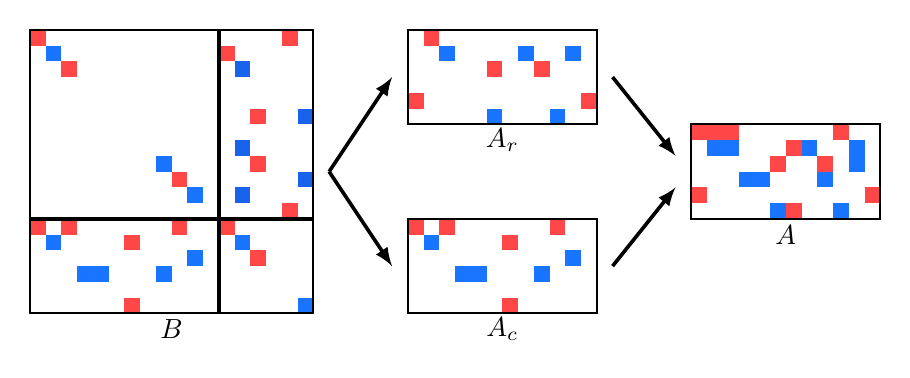
\begin{tikzpicture}[scale=0.2]
\visible<3->{
		\foreach \x / \y in {1/1,1/3,6/7,1/10,2/7}{ \fill[myred] ({42+\y-1},{-\x+1}) rectangle +(1,-1);}
		\foreach \x / \y in {2/2,4/5,4/4,4/9,3/11}{ \fill[myblue] ({42+\y-1},{-\x+1}) rectangle +(1,-1);}
		\foreach \x / \y in {1/2,3/6,3/9,5/1,5/12} { \fill[myred] ({42+\y-1},{-\x+1}) rectangle +(1,-1);}
		\foreach \x / \y in {2/3,6/6,6/10,2/11,2/8} { \fill[myblue] ({42+\y-1},{-\x+1}) rectangle +(1,-1);}
	%\draw[semithick] (42,-6) grid +(12,6);
		\draw[thick] (42,-6) rectangle +(12,6);

		\node at (48,-7) {$A$};
		\draw[myarrow] (37,-9) -- +(4,5);
		\draw[myarrow] (37,3) -- +(4,-5);
	}
	\visible<2->{
		\foreach \x / \y in {1/1,1/3,6/7,1/10,2/7}{ \fill[myred] ({24+\y-1},{-6-\x+1}) rectangle +(1,-1);}
		\foreach \x / \y in {2/2,4/5,4/4,4/9,3/11}{ \fill[myblue] ({24+\y-1},{-6-\x+1}) rectangle +(1,-1);}

		\node at (30,-13) {$A_c$};
	%\draw[semithick] (24,{-6-6}) grid +(12,6);
		\draw[thick] (24,{-6-6}) rectangle +(12,6);

		\foreach \x / \y in {1/2,3/6,3/9,5/1,5/12} { \fill[myred] ({24+\y-1},{6-\x+1}) rectangle +(1,-1);}
		\foreach \x / \y in {2/3,6/6,6/10,2/11,2/8} { \fill[myblue] ({24+\y-1},{6-\x+1}) rectangle +(1,-1);}
		\node at (30,-1) {$A_r$};
	%\draw[semithick] (24,{-6+6}) grid +(12,6);
			\draw[myarrow] (19,-3) -- +(4,6);
		\draw[myarrow] (19,-3) -- +(4,-6);
	\draw[thick] (24,{-6+6}) rectangle +(12,6);
	}

		\foreach \x / \y in {1/1,1/3,6/7,1/10,2/7}{ \fill[myred] ({0+\y-1},{-6-\x+1}) rectangle +(1,-1);}
		\foreach \x / \y in {2/2,4/5,4/4,4/9,3/11}{ \fill[myblue] ({0+\y-1},{-6-\x+1}) rectangle +(1,-1);}

		\foreach \x in {1,3,10} { \fill[myred] ({0+\x-1},{6-\x+1}) rectangle +(1,-1);}
		\foreach \x in {2,9,11} { \fill[myblue] ({0+\x-1},{6-\x+1}) rectangle +(1,-1);}

		\foreach \x / \y in  {1/2,2/3,3/6,3/9,6/6,5/1,5/12,6/10,2/11,2/8} { \fill[myred] ({12+\x-1},{6-\y+1}) rectangle +(1,-1);}
		\foreach \x / \y in  {2/3,6/6,6/10,2/11,2/8} { \fill[myblue] ({12+\x-1},{6-\y+1}) rectangle +(1,-1);}

		\foreach \x in {1,3} { \fill[myred] ({12+\x-1},{-6-\x+1}) rectangle +(1,-1);}
		\foreach \x in {2,6} { \fill[myblue] ({12+\x-1},{-6-\x+1}) rectangle +(1,-1);}

	%\draw[very thin,help lines] (0,-12) grid +(18,18);
		\draw[thick] (0,-12) rectangle +(18,18);
		\draw[ultra thick] (12,-12) -- +(0,18);
		\draw[ultra thick] (0,-6) -- +(18,0);

		\node at (9,-13) {$B$};
	\end{tikzpicture}

\end{figure}

	\visible<2->{
\begin{itemize}
\item Retrieval of $A_r$ and $A_c$ with the new partitioning
	\visible<3->{
\item Reassembling of $A$}
	\end{itemize}
}
\end{frame}

\begin{frame}{Medium grain}

	\begin{figure}
		\centering
		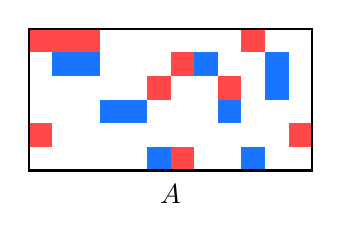
\begin{tikzpicture}[scale=0.3]
			\foreach \x / \y in {1/1,1/3,6/7,1/10,2/7}{ \fill[myred] ({42+\y-1},{-\x+1}) rectangle +(1,-1);}
		\foreach \x / \y in {2/2,4/5,4/4,4/9,3/11}{ \fill[myblue] ({42+\y-1},{-\x+1}) rectangle +(1,-1);}
		\foreach \x / \y in {1/2,3/6,3/9,5/1,5/12} { \fill[myred] ({42+\y-1},{-\x+1}) rectangle +(1,-1);}
		\foreach \x / \y in {2/3,6/6,6/10,2/11,2/8} { \fill[myblue] ({42+\y-1},{-\x+1}) rectangle +(1,-1);}
	%\draw[semithick] (42,-6) grid +(12,6);
		\draw[thick] (42,-6) rectangle +(12,6);

		\node at (48,-7) {$A$};
\end{tikzpicture}

\end{figure}
	\textbf{Clusters} of nonzeros are grouped together: 
	
	\begin{itemize}
		\item in $A_r$ we kept together elements of the same row;
		\item in $A_c$ elements of the same column.
	\end{itemize}

\end{frame}

\begin{frame}{Research directions}

%	Numerical experiments showed that the medium-grain method with \emph{Mondriaan} software partitionare gives good results.

	Two research directions:

\begin{itemize}
	\item Improving the initial partitioning of $A$
	\item Development of a fully iterative scheme: lowering the communication value by using information on the previous partitioning 
\end{itemize}

These directions can be combined: we can try to find efficient ways of splitting $A$ into $A_r$ and $A_c$, distinguishing between

\begin{itemize}
	\item \emph{partition-oblivious} heuristics: no prior information is required
	\item \emph{partition-aware} heuristics: requirement of $A$ already partitioned
\end{itemize}
\end{frame}




\section{Methods}

\subsection{Individual assignment of nonzeros}

\begin{frame}{General remarks}

A few general principles to guide us in the construction of the heuristics:

\begin{itemize}\itemsep=0.5cm
	\item short rows/columns (w.r.t. the number of nonzeros) are more likely to be uncut in a good partitioning 
	\item if a row/column is uncut, the partitioner decided at the previous iteration that it was convenient to do so. 
		
		We shall try to keep, as much as possible, those rows/columns uncut again.

\end{itemize}


\end{frame}

\begin{frame}{Individual assignment of nonzeros}
A simple heuristic is the extension of the original algorithm used in medium-grain.

\emph{Partition-oblivious} version:

\begin{algorithm}[H]
	\begin{algorithmic}
		\ForAll{$a_{ij} \in A$}
		\If{$nz_r(i)<nz_c(j)$}
		\State assign $a_{ij}$ to $A_r$
		\ElsIf{$nz_c(j)<nz_r(i)$}
		\State assign $a_{ij}$ to $A_c$
		\Else
		\State assign $a_{ij}$ to according to tie-breaker
		\EndIf
		\EndFor
	\end{algorithmic}
\end{algorithm}
\end{frame}

\begin{frame}{Individual assignment of nonzeros}

	\begin{figure}[h]
	\centering
	\begin{tikzpicture}[scale=0.5]
		\only<1>{	\foreach \x / \y in {1/1,1/3,1/2} { \fill[myblack] ({\y-1},{-\x+1}) rectangle +(1,-1);} }
		\only<2->{	\foreach \x / \y in {1/1,1/3,1/2} { \fill[mypurple] ({\y-1},{-\x+1}) rectangle +(1,-1);} }
\only<1>{
		\foreach \x / \y in {2/2,2/3,3/6,3/9,6/6,5/1,7/8,8/7,9/2} { \fill[myblack] ({\y-1},{-\x+1}) rectangle +(1,-1);}
		\foreach \x / \y in {4/5,4/4,7/3,8/5,6/7,9/1} { \fill[myblack] ({\y-1},{-\x+1}) rectangle +(1,-1);}
	}
	\only<2->{
		\foreach \x / \y in {2/2,2/3,5/1,7/3,8/7,9/1,9/2} { \fill[mygreen] ({\y-1},{-\x+1}) rectangle +(1,-1);}
		\foreach \x / \y in {3/6,3/9,6/6,4/5,4/4,7/8,8/5,6/7} { \fill[mypurple] ({\y-1},{-\x+1}) rectangle +(1,-1);}
	}
%		\draw[semithick] (0,-9) grid (9,0);
		\draw[thick] (0,-9) rectangle (9,0);
		\fill[mypurple] (13,-4) rectangle (14,-3);
		\fill[mygreen] (13,-6) rectangle (14,-5);
		\node at (15,-3.5) {$A_c$};
		\node at (15,-5.5) {$A_r$};
		\node at (14,-7.5) {tie-breaking: $A_c$};
	\end{tikzpicture}
\end{figure}

\end{frame}


\begin{frame}{Individual assignment of nonzeros}

\emph{Partition-aware} version:

\begin{algorithm}[H]
	\begin{algorithmic}
		\ForAll{$a_{ij} \in A$}
		\If{row $i$ is uncut and column $j$ is cut}
		\State assign $a_{ij}$ to $A_r$
		\ElsIf{row $i$ is cut and column $j$ is uncut}
		\State assign $a_{ij}$ to $A_c$
		\Else
		\State assign $a_{ij}$ as in the partition-oblivious variant
		\EndIf
		\EndFor
	\end{algorithmic}
\end{algorithm}

\end{frame}

\begin{frame}{Individual assignment of nonzeros}

\begin{figure}[h]
	\centering
	\begin{tikzpicture}[scale=0.5]
\only<1>{		\foreach \x / \y in {1/1,1/3,2/2,4/5,4/4,7/3,8/5,6/7,9/1} { \fill[myred] ({\y-1},{-\x+1}) rectangle +(1,-1);}
		\foreach \x / \y in {1/2,2/3,3/6,3/9,6/6,5/1,7/8,8/7,9/2} { \fill[myblue] ({\y-1},{-\x+1}) rectangle +(1,-1);}
	}
\only<2>{		\foreach \x / \y in {1/1,1/3,2/2,7/3,6/7,9/1} { \fill[myred] ({\y-1},{-\x+1}) rectangle +(1,-1);}
		\foreach \x / \y in {1/2,2/3,8/7,9/2} { \fill[myblue] ({\y-1},{-\x+1}) rectangle +(1,-1);}
	}
\only<2->{		\foreach \x / \y in {4/4,3/9,7/8,8/5,6/6} { \fill[mypurple] ({\y-1},{-\x+1}) rectangle +(1,-1);}
		\foreach \x / \y in {4/5,3/6,5/1} { \fill[mygreen] ({\y-1},{-\x+1}) rectangle +(1,-1);}
	}
\only<3->{
	\foreach \x / \y in {1/1,1/3,2/2,7/3,6/7,9/1} { \fill[mygreen] ({\y-1},{-\x+1}) rectangle +(1,-1);}
		\foreach \x / \y in {1/2,2/3,8/7,9/2} { \fill[mygreen] ({\y-1},{-\x+1}) rectangle +(1,-1);}
	}

		\draw[thick] (0,-9) rectangle (9,0);
		\fill[mypurple] (13,-4) rectangle (14,-3);
		\fill[mygreen] (13,-6) rectangle (14,-5);
		\node at (15,-3.5) {$A_c$};
		\node at (15,-5.5) {$A_r$};
		\node at (14,-7.5) {tie-breaking: $A_r$};
	\end{tikzpicture}
\end{figure}
\end{frame}

%\begin{frame}
%%%example
%\begin{figure}[h]
%	\centering
%	\begin{tikzpicture}[scale=0.5]
%		\foreach \x / \y in {1/1,1/3,2/2,4/5,4/4,7/3,8/5,6/7,9/1} { \fill[myred] ({\y-1},{-\x+1}) rectangle +(1,-1);}
%		\foreach \x / \y in {1/2,2/3,3/6,3/9,6/6,5/1,7/8,8/7,9/2} { \fill[myblue] ({\y-1},{-\x+1}) rectangle +(1,-1);}
%%		\draw[semithick] (0,-9) grid (9,0);
%		\draw[thick] (0,-9) rectangle (9,0);
%		\fill[mypurple] (13,-4) rectangle (14,-3);
%		\fill[mygreen] (13,-6) rectangle (14,-5);
%		\node at (15,-3.5) {$A_c$};
%		\node at (15,-5.5) {$A_r$};
%		\node at (14,-7.5) {tie-breaking: $A_c$};
%	\end{tikzpicture}
%\end{figure}
%\end{frame}

\subsection{Assignment of blocks of nonzeros}

\begin{frame}{Assignment of blocks of nonzeros}

	\textbf{Separated Block Diagonal} (SBD) form of a partitioned matrix: we separate uncut and cut rows and columns.
	
	\begin{figure}[h]
	\centering
	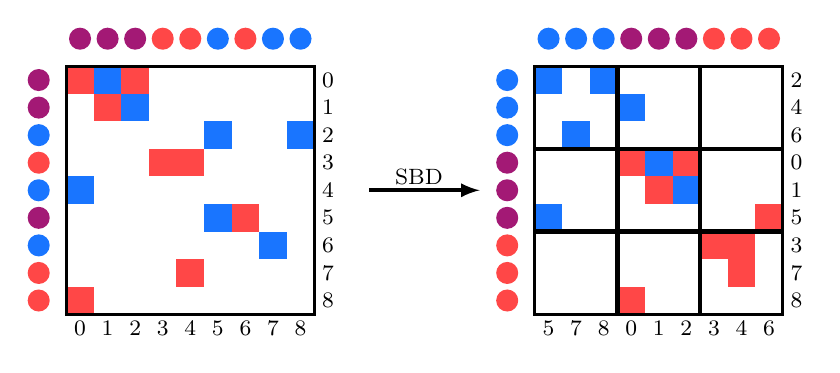
\begin{tikzpicture}[scale=0.35,font=\footnotesize]
		\foreach \x / \y in {1/1,1/3,2/2,4/5,4/4,8/5,6/7,9/1} { \fill[myred] ({\y-1},{-\x+1}) rectangle +(1,-1);}
		\foreach \x / \y in {1/2,2/3,3/6,3/9,6/6,5/1,7/8} { \fill[myblue] ({\y-1},{-\x+1}) rectangle +(1,-1);}
%		\draw[help lines] (0,-9) grid (9,0);
		\foreach \x in {0,1,...,8} {\node at ({9.5},{-\x-.5}) {\x};}
		\foreach \x in {0,1,...,8} {\node at ({\x+.5},-9.5) {\x};}


		\foreach \x in {1,2,3} { \fill[mypurple] ({\x-0.5},1) circle (0.4cm);}
		\foreach \x in {4,5,7} { \fill[myred] ({\x-0.5},1) circle (0.4cm);}
		\foreach \x in {6,8,9} { \fill[myblue] ({\x-0.5},1) circle (0.4cm);}

		\foreach \x in {1,2,6} { \fill[mypurple] (-1,{-\x+0.5}) circle (0.4cm);}
		\foreach \x in {4,8,9} { \fill[myred] (-1,{-\x+0.5}) circle (0.4cm);}
		\foreach \x in {3,5,7} { \fill[myblue] (-1,{-\x+0.5}) circle (0.4cm);}

		\draw[very thick] (0,-9) rectangle (9,0);

		\draw[thick,myarrow] (11,-4.5) -- (15,-4.5);
		\node at (12.8,-4) {SBD};
		\foreach \x / \y in {4/4,4/6,5/5,7/8,7/7,8/8,6/9,9/4} { \fill[myred] ({17+\y-1},{-\x+1}) rectangle +(1,-1);}
		\foreach \x / \y in {1/1,1/3,2/4,3/2,4/5,5/6,6/1} { \fill[myblue] ({17+\y-1},{-\x+1}) rectangle +(1,-1);}

%		\draw[help lines] (17,-9) grid ({17+9},0);
		\foreach \x / \y in {2/0,4/1,6/2,0/3,1/4,5/5,3/6,7/7,8/8} {\node at ({17+9.5},{-\y-.5}) {\x};}
		\foreach \x / \y in {5/0,7/1,8/2,0/3,1/4,2/5,3/6,4/7,6/8} {\node at ({17+\y+.5},-9.5) {\x};}


		\foreach \x in {4,5,6} { \fill[mypurple] ({17+\x-0.5},1) circle (0.4cm);}
		\foreach \x in {7,8,9} { \fill[myred] ({17+\x-0.5},1) circle (0.4cm);}
		\foreach \x in {1,2,3} { \fill[myblue] ({17+\x-0.5},1) circle (0.4cm);}

		\foreach \x in {4,5,6} { \fill[mypurple] ({17-1},{-\x+0.5}) circle (0.4cm);}
		\foreach \x in {7,8,9} { \fill[myred] ({17-1},{-\x+0.5}) circle (0.4cm);}
		\foreach \x in {1,2,3} { \fill[myblue] ({17-1},{-\x+0.5}) circle (0.4cm);}

		\draw[very thick] ({17+0},-9) rectangle ({17+9},0);

		\draw[ultra thick] ({17+3},0) -- ({17+3},-9);
		\draw[ultra thick] ({17+6},0) -- ({17+6},-9);

		\draw[ultra thick] ({17+0},-3) -- ({17+9},-3);
		\draw[ultra thick] ({17+0},-6) -- ({17+9},-6);
	\end{tikzpicture}
\end{figure}

\end{frame}

\begin{frame}{Assignment of blocks of nonzeros}

	\begin{minipage}{6cm}
	\begin{figure}[h]
	\centering
	\begin{tikzpicture}[scale=0.35,font=\footnotesize]
\only<1>{			\foreach \x / \y in {4/4,4/6,5/5,7/8,7/7,8/8,6/9,9/4} { \fill[myred] ({17+\y-1},{-\x+1}) rectangle +(1,-1);}
		\foreach \x / \y in {1/1,1/3,2/4,3/2,4/5,5/6,6/1} { \fill[myblue] ({17+\y-1},{-\x+1}) rectangle +(1,-1);}
	}	
\only<2>{
		\foreach \x / \y in {6/1,6/9,7/7,7/8,8/8,4/4,4/5,4/6} { \fill[mypurple] ({17+\y-1},{-\x+1}) rectangle +(1,-1);}
		\foreach \x / \y in {2/4,9/4,1/1,1/3,3/2,5/5,5/6} { \fill[mygreen] ({17+\y-1},{-\x+1}) rectangle +(1,-1);}
	}
%		\draw[help lines] (17,-9) grid ({17+9},0);
		\draw[very thick] ({17+0},-9) rectangle ({17+9},0);

		\draw[ultra thick] ({17+3},0) -- ({17+3},-9);
		\draw[ultra thick] ({17+6},0) -- ({17+6},-9);

		\draw[ultra thick] ({17+0},-3) -- ({17+9},-3);
		\draw[ultra thick] ({17+0},-6) -- ({17+9},-6);
	\end{tikzpicture}
\end{figure}
\end{minipage}
\begin{minipage}{4cm}

\only<1>{
The SBD form is a $3 \times 3$ block matrix

\begin{align*}  
	\begin{bmatrix}
		\dot{A}_{00} & \dot{A}_{01}  & \\
		\dot{A}_{10} & \dot{A}_{11} & \dot{A}_{12} \\
		& \dot{A}_{21} & \dot{A}_{22} \\ 
	\end{bmatrix}
\end{align*}}
\only<2>{
\begin{align*}
\begin{bmatrix}
		A_r/A_c & A_r & \\
		A_c & M & A_c \\
		& A_r & A_r/A_c \\
	\end{bmatrix}
\end{align*}
\vspace{-0.25cm}
\begin{figure}[h]
	\centering
	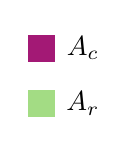
\begin{tikzpicture}[scale=0.35]
		\fill[mypurple] (13,-4) rectangle (14,-3);
		\fill[mygreen] (13,-6) rectangle (14,-5);
		\node at (15,-3.5) {$A_c$};
		\node at (15,-5.5) {$A_r$};
	\end{tikzpicture}
\end{figure}

}
\end{minipage}

\vspace{0.5cm}

$\dot{A}_{01}$, $\dot{A}_{10}$, $\dot{A}_{12}$, $\dot{A}_{21}$ can be easily assigned in our framework.
\visible<2->{\begin{itemize}
	\item $A_r/A_c$ means that the size of the block determines whether it is assigned to $A_r$ or $A_c$;
	\item the nonzeros in the middle block are assigned individually ($M$ stands for ``mixed'' assignment)
\end{itemize}
}
\end{frame}

\begin{frame}{Assignment of blocks of nonzeros}
	\begin{figure}[h]
	\centering
	\begin{tikzpicture}[scale=0.5]
\only<1>{		\foreach \x / \y in {6/1,6/9,7/7,7/8,8/8,4/4,4/5,4/6} { \fill[mypurple] ({17+\y-1},{-\x+1}) rectangle +(1,-1);}
		\foreach \x / \y in {2/4,9/4,1/1,1/3,3/2,5/5,5/6} { \fill[mygreen] ({17+\y-1},{-\x+1}) rectangle +(1,-1);}

%		\draw[help lines] (17,-9) grid ({17+9},0);
		\foreach \x / \y in {2/0,4/1,6/2,0/3,1/4,5/5,3/6,7/7,8/8} {\node at ({17+9.5},{-\y-.5}) {\x};}
		\foreach \x / \y in {5/0,7/1,8/2,0/3,1/4,2/5,3/6,4/7,6/8} {\node at ({17+\y+.5},-9.5) {\x};}

		\draw[very thick] ({17+0},-9) rectangle ({17+9},0);

		\draw[ultra thick] ({17+3},0) -- ({17+3},-9);
		\draw[ultra thick] ({17+6},0) -- ({17+6},-9);

		\draw[ultra thick] ({17+0},-3) -- ({17+9},-3);
		\draw[ultra thick] ({17+0},-6) -- ({17+9},-6);}

\only<2>{	
		\foreach \x / \y in {1/1,1/3,1/2,4/5,4/4,8/5,6/7,6/6} { \fill[mypurple] ({17+\y-1},{-\x+1}) rectangle +(1,-1);}
		\foreach \x / \y in {2/2,2/3,3/6,3/9,5/1,7/8,9/1} { \fill[mygreen] ({17+\y-1},{-\x+1}) rectangle +(1,-1);}

%		\draw[help lines] (17,-9) grid ({17+9},0);
		\foreach \x / \y in {0/0,1/1,2/2,3/3,4/4,5/5,6/6,7/7,8/8} {\node at ({17+9.5},{-\y-.5}) {\x};}
		\foreach \x / \y in {0/0,1/1,2/2,3/3,4/4,5/5,6/6,7/7,8/8} {\node at ({17+\y+.5},-9.5) {\x};}

		\draw[very thick] ({17+0},-9) rectangle ({17+9},0);
	}
	\end{tikzpicture}
\end{figure}
\visible<2->{
\begin{itemize}
	\item We reverse the permutations of rows and columns, obtaining $A$ back, with new assignment.
\end{itemize}
}
\end{frame}

\begin{frame}{Assignment of blocks of nonzeros}

	\textbf{Separated Block Diagonal} form of order 2 (SBD2) of a matrix: we split the top, bottom, left and right blocks, separating the empty and nonempty parts.

	\begin{figure}[h]
	\centering
	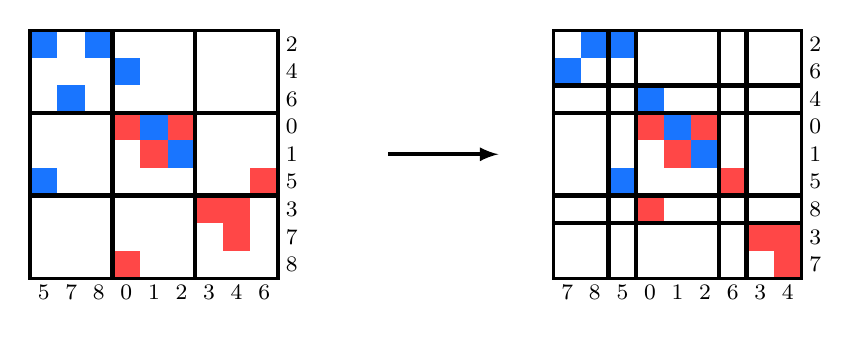
\begin{tikzpicture}[scale=0.35,font=\footnotesize]
		\foreach \x / \y in {4/4,4/6,5/5,7/8,7/7,8/8,6/9,9/4} { \fill[myred] ({0+\y-1},{-\x+1}) rectangle +(1,-1);}
		\foreach \x / \y in {1/1,1/3,2/4,3/2,4/5,5/6,6/1} { \fill[myblue] ({0+\y-1},{-\x+1}) rectangle +(1,-1);}

%		\draw[help lines] (0,-9) grid ({0+9},0);
		\foreach \x / \y in {2/0,4/1,6/2,0/3,1/4,5/5,3/6,7/7,8/8} {\node at ({0+9.5},{-\y-.5}) {\x};}
		\foreach \x / \y in {5/0,7/1,8/2,0/3,1/4,2/5,3/6,4/7,6/8} {\node at ({0+\y+.5},-9.5) {\x};}

%		\node at (1.5,-10.7) {$C_0$};
%		\node at (4.5,-10.7) {$C_1$};
%		\node at (7.5,-10.7) {$C_2$};
%
%		\node at (11,-1.5) {$R_0$};
%		\node at (11,-4.5) {$R_1$};
%		\node at (11,-7.5) {$R_2$};

		\draw[very thick] ({0+0},-9) rectangle ({0+9},0);

		\draw[ultra thick] ({0+3},0) -- ({0+3},-9);
		\draw[ultra thick] ({0+6},0) -- ({0+6},-9);

		\draw[ultra thick] ({0+0},-3) -- ({0+9},-3);
		\draw[ultra thick] ({0+0},-6) -- ({0+9},-6);

		\draw[thick,myarrow] (13,-4.5) -- (17,-4.5);

		\foreach \x / \y in {4/4,4/6,5/5,8/9,8/8,9/9,6/7,7/4} { \fill[myred] ({19+\y-1},{-\x+1}) rectangle +(1,-1);}
		\foreach \x / \y in {1/3,1/2,3/4,2/1,4/5,5/6,6/3} { \fill[myblue] ({19+\y-1},{-\x+1}) rectangle +(1,-1);}

%		\draw[help lines] (19,-9) grid ({19+9},0);
		\foreach \x / \y in {2/0,6/1,4/2,0/3,1/4,5/5,8/6,3/7,7/8} {\node at ({19+9.5},{-\y-.5}) {\x};}
		\foreach \x / \y in {7/0,8/1,5/2,0/3,1/4,2/5,6/6,3/7,4/8} {\node at ({19+\y+.5},-9.5) {\x};}

%		\node at ({19+1},-10.7) {$C_{00}$};
%		\node at ({19+2.5},-10.7) {$C_{01}$};
%		\node at ({19+4.5},-10.7) {$C_{1}$};
%		\node at ({19+6.5},-10.7) {$C_{20}$};
%		\node at ({19+8},-10.7) {$C_{21}$};
%
%		\node at ({19+11},-1) {$R_{00}$};
%		\node at ({19+11},-2.5) {$R_{01}$};
%		\node at ({19+11},-4.5) {$R_{1}$};
%		\node at ({19+11},-6.5) {$R_{20}$};
%		\node at ({19+11},-8) {$R_{21}$};

		\draw[very thick] ({19+0},-9) rectangle ({19+9},0);

		\draw[ultra thick] ({19+3},0) -- ({19+3},-9);
		\draw[ultra thick] ({19+6},0) -- ({19+6},-9);
		\draw[ultra thick] ({19+2},0) -- ({19+2},-9);
		\draw[ultra thick] ({19+7},0) -- ({19+7},-9);

		\draw[ultra thick] ({19+0},-3) -- ({19+9},-3);
		\draw[ultra thick] ({19+0},-6) -- ({19+9},-6);
		\draw[ultra thick] ({19+0},-2) -- ({19+9},-2);
		\draw[ultra thick] ({19+0},-7) -- ({19+9},-7);
	\end{tikzpicture}
\end{figure}

\end{frame}


\begin{frame}{Assignment of blocks of nonzeros}
	\begin{minipage}{5.5cm}
	\begin{figure}[h]
	\centering
	\begin{tikzpicture}[scale=0.35,font=\footnotesize]
\only<1>{
		\foreach \x / \y in {4/4,4/6,5/5,8/9,8/8,9/9,6/7,7/4} { \fill[myred] ({19+\y-1},{-\x+1}) rectangle +(1,-1);}
		\foreach \x / \y in {1/3,1/2,3/4,2/1,4/5,5/6,6/3} { \fill[myblue] ({19+\y-1},{-\x+1}) rectangle +(1,-1);}
	}
		\only<2->{
		\foreach \x / \y in {6/3,4/4,4/5,4/6,6/7,8/8,8/9,9/9} { \fill[mypurple] ({19+\y-1},{-\x+1}) rectangle +(1,-1);}
		\foreach \x / \y in {1/2,1/3,2/1,3/4,7/4,5/5,5/6} { \fill[mygreen] ({19+\y-1},{-\x+1}) rectangle +(1,-1);}
	}
		\draw[very thick] ({19+0},-9) rectangle ({19+9},0);

		\draw[ultra thick] ({19+3},0) -- ({19+3},-9);
		\draw[ultra thick] ({19+6},0) -- ({19+6},-9);
		\draw[ultra thick] ({19+2},0) -- ({19+2},-9);
		\draw[ultra thick] ({19+7},0) -- ({19+7},-9);

		\draw[ultra thick] ({19+0},-3) -- ({19+9},-3);
		\draw[ultra thick] ({19+0},-6) -- ({19+9},-6);
		\draw[ultra thick] ({19+0},-2) -- ({19+9},-2);
		\draw[ultra thick] ({19+0},-7) -- ({19+9},-7);
	\end{tikzpicture}
\end{figure}

\end{minipage}
\begin{minipage}{4cm}
\only<1>{
	The SBD2 form of a matrix is the following $5 \times 5$ block matrix:

	\begin{align*}
	\begin{bmatrix}
		\ddot{A}_{00} & \ddot{A}_{01} & & & \\
		\ddot{A}_{10} & \ddot{A}_{11} & \ddot{A}_{12} & & \\
		& \ddot{A}_{21} & \ddot{A}_{22} & \ddot{A}_{23} & \\
		& & \ddot{A}_{32} & \ddot{A}_{33} & \ddot{A}_{34} \\
		& & & \ddot{A}_{43} & \ddot{A}_{44} \\
	\end{bmatrix}
\end{align*}
}
\only<2->{
\begin{align*}
	\begin{bmatrix}
		A_r & A_r & & & \\
		A_c & A_r/A_c & A_r & & \\
		& A_c & M & A_c & \\
		& & A_r & A_r/A_c & A_c \\
		& & & A_r & A_c \\
	\end{bmatrix}
\end{align*}

\vspace{-0.25cm}

\begin{figure}[h]
	\centering
	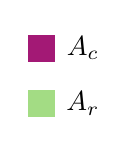
\begin{tikzpicture}[scale=0.35]
		\fill[mypurple] (13,-4) rectangle (14,-3);
		\fill[mygreen] (13,-6) rectangle (14,-5);
		\node at (15,-3.5) {$A_c$};
		\node at (15,-5.5) {$A_r$};
	\end{tikzpicture}
\end{figure}

}

\end{minipage}

\vspace{0.4cm}

In this form, other than having information on nonzeros (rows/columns cut/uncut), we also have information on their neighbors (nonzeros in the same row and column).

\end{frame}


\begin{frame}{Individual assignment of blocks of nonzeros}
	\begin{figure}[h]
	\centering
	\begin{tikzpicture}[scale=0.5]
		\only<1>{ \foreach \x / \y in {6/3,4/4,4/5,4/6,6/7,8/8,8/9,9/9} { \fill[mypurple] ({19+\y-1},{-\x+1}) rectangle +(1,-1);}
		\foreach \x / \y in {1/2,1/3,2/1,3/4,7/4,5/5,5/6} { \fill[mygreen] ({19+\y-1},{-\x+1}) rectangle +(1,-1);}

		\draw[ultra thick] ({19+3},0) -- ({19+3},-9);
		\draw[ultra thick] ({19+6},0) -- ({19+6},-9);
		\draw[ultra thick] ({19+2},0) -- ({19+2},-9);
		\draw[ultra thick] ({19+7},0) -- ({19+7},-9);
		\foreach \x / \y in {2/0,6/1,4/2,0/3,1/4,5/5,8/6,3/7,7/8} {\node at ({19+9.5},{-\y-.5}) {\x};}
		\foreach \x / \y in {7/0,8/1,5/2,0/3,1/4,2/5,6/6,3/7,4/8} {\node at ({19+\y+.5},-9.5) {\x};}


		\draw[ultra thick] ({19+0},-3) -- ({19+9},-3);
		\draw[ultra thick] ({19+0},-6) -- ({19+9},-6);
		\draw[ultra thick] ({19+0},-2) -- ({19+9},-2);
		\draw[ultra thick] ({19+0},-7) -- ({19+9},-7);
	}
\only<2>{	
		\foreach \x / \y in {1/1,1/3,1/2,4/5,4/4,8/5,6/7,6/6} { \fill[mypurple] ({19+\y-1},{-\x+1}) rectangle +(1,-1);}
		\foreach \x / \y in {2/2,2/3,3/6,3/9,5/1,7/8,9/1} { \fill[mygreen] ({19+\y-1},{-\x+1}) rectangle +(1,-1);}
		\foreach \x / \y in {0/0,1/1,2/2,3/3,4/4,5/5,6/6,7/7,8/8} {\node at ({19+9.5},{-\y-.5}) {\x};}
		\foreach \x / \y in {0/0,1/1,2/2,3/3,4/4,5/5,6/6,7/7,8/8} {\node at ({19+\y+.5},-9.5) {\x};}
	}

		\draw[very thick] ({19+0},-9) rectangle ({19+9},0);
	
	\end{tikzpicture}
\end{figure}
\visible<2->{
\begin{itemize}
	\item We reverse the permutations of rows and columns, obtaining $A$ back, with new assignment.
\end{itemize}
}
\end{frame}
\subsection{Partial assignment of rows and columns}

\begin{frame}{Partial assignment of rows and columns}

\begin{itemize}
		\item	Main idea: Every time we assign a nonzero to either $A_r$ or $A_c$, all the other nonzeros in the same row/column should be assigned to it as well, to prevent communication.
		\item	Main issue: Hard to assign complete rows/column: a nonzero cannot be assigned to both $A_r$ and $A_c$.
\end{itemize}

We need to reason in terms of \textbf{partial assignment}:

	\begin{itemize}
		\item	computation of a \textbf{priority vector}:
			
			a permutation of the indices $\{0,\dots,m+n-1\}$ (decreasing priority) 
			\begin{itemize}
				\item  $\{0,\dots,m-1\}$ correspond to rows;
				\item  $\{m,\dots,m+n-1\}$ to columns.
			\end{itemize}
		\item \textbf{overpainting algorithm}.
	\end{itemize}
\end{frame}


\begin{frame}{Overpainting algorithm}
\begin{algorithm}[H]
	\begin{algorithmic}
		\Require{Priority vector $v$, matrix $A$}
		\Ensure{$A_r$, $A_c$}
		\State $A_r := A_c: = \varnothing$
		\For{$i=m+n-1,\dots,0$}
	\If{$v_i < m$}
	\State Add the nonzeros of row $i$ to $A_r$
	\Else
	\State Add the nonzeros of column $i-m$ to $A_c$
	\EndIf
	\EndFor
\end{algorithmic}
\end{algorithm}

\vspace{-0.4cm}

\begin{itemize}
	\item In this formulation of the algorithm, every nonzero is assigned twice;
	\item the algorithm is \textbf{completely deterministic}: $A_r$ and $A_c$ depend entirely on the priority vector $v$.
\end{itemize}

\end{frame}

\begin{frame}{Overpainting algorithm}

Example:
let $v := \{\alt<19>{\textcolor{red}{0}}{0},
\alt<18>{\textcolor{red}{9}}{9},
\alt<17>{\textcolor{red}{1}}{1},
\alt<16>{\textcolor{red}{10}}{10},
\alt<15>{\textcolor{red}{2}}{2},
\alt<14>{\textcolor{red}{11}}{11},
\alt<13>{\textcolor{red}{3}}{3},
\alt<12>{\textcolor{red}{12}}{12},
\alt<11>{\textcolor{red}{4}}{4},
\alt<10>{\textcolor{red}{13}}{13},
\alt<9>{\textcolor{red}{5}}{5},
\alt<8>{\textcolor{red}{14}}{14},
\alt<7>{\textcolor{red}{6}}{6},
\alt<6>{\textcolor{red}{15}}{15},
\alt<5>{\textcolor{red}{7}}{7},
\alt<4>{\textcolor{red}{16}}{16},
\alt<3>{\textcolor{red}{8}}{8},
\alt<2>{\textcolor{red}{17}}{17}\}$

\begin{figure}[h]
\centering
\begin{tikzpicture}[scale=0.5]
	\only<1>{
	\foreach \x / \y in {1/1,1/3,2/2,4/5,4/4,7/3,8/5,6/7,9/1} { \fill[myred] ({\y-1},{-\x+1}) rectangle +(1,-1);}
	\foreach \x / \y in {1/2,2/3,3/6,3/9,6/6,5/1,7/8,8/7,9/2} { \fill[myblue] ({\y-1},{-\x+1}) rectangle +(1,-1);}
}
	\only<2>{
	\foreach \x / \y in {1/1,1/3,2/2,4/5,4/4,7/3,8/5,6/7,9/1} { \fill[myred] ({\y-1},{-\x+1}) rectangle +(1,-1);}
	\foreach \x / \y in {1/2,2/3,3/6,6/6,5/1,7/8,8/7,9/2} { \fill[myblue] ({\y-1},{-\x+1}) rectangle +(1,-1);}
	\foreach \x / \y in {3/9} { \fill[mypurple] ({\y-1},{-\x+1}) rectangle +(1,-1);}
	\foreach \x / \y in {} { \fill[mygreen] ({\y-1},{-\x+1}) rectangle +(1,-1);}
}
	\only<3>{
	\foreach \x / \y in {1/1,1/3,2/2,4/5,4/4,7/3,8/5,6/7} { \fill[myred] ({\y-1},{-\x+1}) rectangle +(1,-1);}
	\foreach \x / \y in {1/2,2/3,3/6,6/6,5/1,7/8,8/7} { \fill[myblue] ({\y-1},{-\x+1}) rectangle +(1,-1);}
	\foreach \x / \y in {3/9} { \fill[mypurple] ({\y-1},{-\x+1}) rectangle +(1,-1);}
	\foreach \x / \y in {9/1,9/2} { \fill[mygreen] ({\y-1},{-\x+1}) rectangle +(1,-1);}
}
	\only<4>{
	\foreach \x / \y in {1/1,1/3,2/2,4/5,4/4,7/3,8/5,6/7} { \fill[myred] ({\y-1},{-\x+1}) rectangle +(1,-1);}
	\foreach \x / \y in {1/2,2/3,3/6,6/6,5/1,8/7} { \fill[myblue] ({\y-1},{-\x+1}) rectangle +(1,-1);}
	\foreach \x / \y in {3/9,7/8} { \fill[mypurple] ({\y-1},{-\x+1}) rectangle +(1,-1);}
	\foreach \x / \y in {9/1,9/2} { \fill[mygreen] ({\y-1},{-\x+1}) rectangle +(1,-1);}
}
	\only<5>{
	\foreach \x / \y in {1/1,1/3,2/2,4/5,4/4,7/3,6/7} { \fill[myred] ({\y-1},{-\x+1}) rectangle +(1,-1);}
	\foreach \x / \y in {1/2,2/3,3/6,6/6,5/1} { \fill[myblue] ({\y-1},{-\x+1}) rectangle +(1,-1);}
	\foreach \x / \y in {3/9,7/8} { \fill[mypurple] ({\y-1},{-\x+1}) rectangle +(1,-1);}
	\foreach \x / \y in {9/1,9/2,8/7,8/5} { \fill[mygreen] ({\y-1},{-\x+1}) rectangle +(1,-1);}
}
	\only<6>{
	\foreach \x / \y in {1/1,1/3,2/2,4/5,4/4,7/3} { \fill[myred] ({\y-1},{-\x+1}) rectangle +(1,-1);}
	\foreach \x / \y in {1/2,2/3,3/6,6/6,5/1} { \fill[myblue] ({\y-1},{-\x+1}) rectangle +(1,-1);}
	\foreach \x / \y in {3/9,7/8,6/7,8/7} { \fill[mypurple] ({\y-1},{-\x+1}) rectangle +(1,-1);}
	\foreach \x / \y in {9/1,9/2,8/5} { \fill[mygreen] ({\y-1},{-\x+1}) rectangle +(1,-1);}
}
	\only<7>{
	\foreach \x / \y in {1/1,1/3,2/2,4/5,4/4} { \fill[myred] ({\y-1},{-\x+1}) rectangle +(1,-1);}
	\foreach \x / \y in {1/2,2/3,3/6,6/6,5/1} { \fill[myblue] ({\y-1},{-\x+1}) rectangle +(1,-1);}
	\foreach \x / \y in {3/9,6/7,8/7} { \fill[mypurple] ({\y-1},{-\x+1}) rectangle +(1,-1);}
	\foreach \x / \y in {9/1,9/2,8/5,7/8,7/3} { \fill[mygreen] ({\y-1},{-\x+1}) rectangle +(1,-1);}
}
	\only<8>{
	\foreach \x / \y in {1/1,1/3,2/2,4/5,4/4} { \fill[myred] ({\y-1},{-\x+1}) rectangle +(1,-1);}
	\foreach \x / \y in {1/2,2/3,5/1} { \fill[myblue] ({\y-1},{-\x+1}) rectangle +(1,-1);}
	\foreach \x / \y in {3/9,6/7,8/7,3/6,6/6} { \fill[mypurple] ({\y-1},{-\x+1}) rectangle +(1,-1);}
	\foreach \x / \y in {9/1,9/2,8/5,7/8,7/3} { \fill[mygreen] ({\y-1},{-\x+1}) rectangle +(1,-1);}
}
	\only<9>{
	\foreach \x / \y in {1/1,1/3,2/2,4/5,4/4} { \fill[myred] ({\y-1},{-\x+1}) rectangle +(1,-1);}
	\foreach \x / \y in {1/2,2/3,5/1} { \fill[myblue] ({\y-1},{-\x+1}) rectangle +(1,-1);}
	\foreach \x / \y in {3/9,8/7,3/6} { \fill[mypurple] ({\y-1},{-\x+1}) rectangle +(1,-1);}
	\foreach \x / \y in {9/1,9/2,8/5,7/8,7/3,6/6,6/7} { \fill[mygreen] ({\y-1},{-\x+1}) rectangle +(1,-1);}
}
	\only<10>{
	\foreach \x / \y in {1/1,1/3,2/2,4/4} { \fill[myred] ({\y-1},{-\x+1}) rectangle +(1,-1);}
	\foreach \x / \y in {1/2,2/3,5/1} { \fill[myblue] ({\y-1},{-\x+1}) rectangle +(1,-1);}
	\foreach \x / \y in {3/9,8/7,3/6,4/5,8/5} { \fill[mypurple] ({\y-1},{-\x+1}) rectangle +(1,-1);}
	\foreach \x / \y in {9/1,9/2,7/8,7/3,6/6,6/7} { \fill[mygreen] ({\y-1},{-\x+1}) rectangle +(1,-1);}
}
	\only<11>{
	\foreach \x / \y in {1/1,1/3,2/2,4/4} { \fill[myred] ({\y-1},{-\x+1}) rectangle +(1,-1);}
	\foreach \x / \y in {1/2,2/3} { \fill[myblue] ({\y-1},{-\x+1}) rectangle +(1,-1);}
	\foreach \x / \y in {3/9,8/7,3/6,4/5,8/5} { \fill[mypurple] ({\y-1},{-\x+1}) rectangle +(1,-1);}
	\foreach \x / \y in {9/1,9/2,7/8,7/3,6/6,6/7,5/1} { \fill[mygreen] ({\y-1},{-\x+1}) rectangle +(1,-1);}
}
	\only<12>{
	\foreach \x / \y in {1/1,1/3,2/2} { \fill[myred] ({\y-1},{-\x+1}) rectangle +(1,-1);}
	\foreach \x / \y in {1/2,2/3} { \fill[myblue] ({\y-1},{-\x+1}) rectangle +(1,-1);}
	\foreach \x / \y in {3/9,8/7,3/6,4/5,8/5,4/4} { \fill[mypurple] ({\y-1},{-\x+1}) rectangle +(1,-1);}
	\foreach \x / \y in {9/1,9/2,7/8,7/3,6/6,6/7,5/1} { \fill[mygreen] ({\y-1},{-\x+1}) rectangle +(1,-1);}
}
	\only<13>{
	\foreach \x / \y in {1/1,1/3,2/2} { \fill[myred] ({\y-1},{-\x+1}) rectangle +(1,-1);}
	\foreach \x / \y in {1/2,2/3} { \fill[myblue] ({\y-1},{-\x+1}) rectangle +(1,-1);}
	\foreach \x / \y in {3/9,8/7,3/6,8/5} { \fill[mypurple] ({\y-1},{-\x+1}) rectangle +(1,-1);}
	\foreach \x / \y in {9/1,9/2,7/8,7/3,6/6,6/7,5/1,4/4,4/5} { \fill[mygreen] ({\y-1},{-\x+1}) rectangle +(1,-1);}
}
	\only<14>{
	\foreach \x / \y in {1/1,2/2} { \fill[myred] ({\y-1},{-\x+1}) rectangle +(1,-1);}
	\foreach \x / \y in {1/2} { \fill[myblue] ({\y-1},{-\x+1}) rectangle +(1,-1);}
	\foreach \x / \y in {3/9,8/7,3/6,8/5,2/3,1/3,7/3} { \fill[mypurple] ({\y-1},{-\x+1}) rectangle +(1,-1);}
	\foreach \x / \y in {9/1,9/2,7/8,6/6,6/7,5/1,4/4,4/5} { \fill[mygreen] ({\y-1},{-\x+1}) rectangle +(1,-1);}
}
	\only<15>{
	\foreach \x / \y in {1/1,2/2} { \fill[myred] ({\y-1},{-\x+1}) rectangle +(1,-1);}
	\foreach \x / \y in {1/2} { \fill[myblue] ({\y-1},{-\x+1}) rectangle +(1,-1);}
	\foreach \x / \y in {8/7,8/5,2/3,1/3,7/3} { \fill[mypurple] ({\y-1},{-\x+1}) rectangle +(1,-1);}
	\foreach \x / \y in {9/1,9/2,7/8,6/6,6/7,5/1,4/4,4/5,3/9,3/6} { \fill[mygreen] ({\y-1},{-\x+1}) rectangle +(1,-1);}
}
	\only<16>{
	\foreach \x / \y in {1/1} { \fill[myred] ({\y-1},{-\x+1}) rectangle +(1,-1);}
	\foreach \x / \y in {8/7,8/5,2/3,1/3,7/3,1/2,2/2,9/2} { \fill[mypurple] ({\y-1},{-\x+1}) rectangle +(1,-1);}
	\foreach \x / \y in {9/1,7/8,6/6,6/7,5/1,4/4,4/5,3/9,3/6} { \fill[mygreen] ({\y-1},{-\x+1}) rectangle +(1,-1);}
}
	\only<17>{
	\foreach \x / \y in {1/1} { \fill[myred] ({\y-1},{-\x+1}) rectangle +(1,-1);}
	\foreach \x / \y in {8/7,8/5,1/3,7/3,1/2,9/2} { \fill[mypurple] ({\y-1},{-\x+1}) rectangle +(1,-1);}
	\foreach \x / \y in {9/1,7/8,6/6,6/7,5/1,4/4,4/5,3/9,3/6,2/2,2/3} { \fill[mygreen] ({\y-1},{-\x+1}) rectangle +(1,-1);}
}
	\only<18>{
	\foreach \x / \y in {8/7,8/5,1/3,7/3,1/2,9/2,1/1,9/1,5/1} { \fill[mypurple] ({\y-1},{-\x+1}) rectangle +(1,-1);}
	\foreach \x / \y in {7/8,6/6,6/7,4/4,4/5,3/9,3/6,2/2,2/3} { \fill[mygreen] ({\y-1},{-\x+1}) rectangle +(1,-1);}
}
	\only<19>{
	\foreach \x / \y in {8/7,8/5,7/3,9/2,9/1,5/1} { \fill[mypurple] ({\y-1},{-\x+1}) rectangle +(1,-1);}
	\foreach \x / \y in {7/8,6/6,6/7,4/4,4/5,3/9,3/6,2/2,2/3,1/1,1/2,1/3} { \fill[mygreen] ({\y-1},{-\x+1}) rectangle +(1,-1);}
}

\foreach \x / \y in {0/2,1/4,2/6,3/8,4/10,5/12,6/14,7/16,8/18} {  \visible<\y>{\draw[line width=2pt,->,>=latex] ({8-\x+0.5},1.8) -- ({8-\x+0.5},0.2);}	}
	\foreach \x / \y in {0/3,1/5,2/7,3/9,4/11,5/13,6/15,7/17,8/19} {  \visible<\y>{\draw[line width=2pt,->,>=latex] (-1.8,{-9+\x+0.5}) -- (-0.2,{-9+\x+0.5});}	}
		\draw[thick] (0,-9) rectangle (9,0);
		\fill[mypurple] (13,-4) rectangle (14,-3);
		\fill[mygreen] (13,-6) rectangle (14,-5);
		\node at (15,-3.5) {$A_c$};
		\node at (15,-5.5) {$A_r$};
	\end{tikzpicture}
\end{figure}
\end{frame}


\begin{frame}{Computation of the priority vector $v$}

We used a structured approach for the construction of $v$: 30 different heuristics.

Generating schemes with three steps:

\begin{enumerate}
	\item Usage of previous partitioning
\visible<2>{		\begin{itemize}
		\item partition-oblivious
	\item partition-aware }
	\end{itemize}
	\item Sorting (w.r.t the number of nonzeros, in ascending order)
\visible<3>{		\begin{itemize}
			\item sorted (with or without refinement)
			\item unsorted
		\end{itemize}
	}
	\item Internal order of indices
\visible<4>{		\begin{itemize}
			\item concatenation
			\item mixing (either alternation or spread)
			\item random (only when not sorting)
			\item simple (only when sorting)
		\end{itemize}
	}
\end{enumerate}

\end{frame}



\section{Independent set formulation}

\begin{frame}{Independent set formulation}

Partial assignment of rows and columns seems an interesting idea, but we want to reduce, as much as possible, the number of cut rows/columns.

\vspace{0.3cm}

\textbf{Goal}: Find the biggest subset of $\{0,\dots,m+n-1\}$ which can be assigned completely (i.e. full rows and full columns) without causing communication.

\vspace{0.3cm}

Graph theory approach: translating the sparsity pattern of $A$ in a particular way, we are looking for a \textbf{maximum independent set}.

\end{frame}

\begin{frame}{Construction of the graph}
	We construct the bipartite graph $G=(L \cup R,E)$ as follows:

\begin{itemize}\itemsep=0.3cm
		\item Rows and columns are vertices
		\begin{itemize}\itemsep=0.2cm
			\item $L = \{r_0,\dots,r_{m-1}\}$
		\item $R = \{c_0,\dots,c_{n-1}\}$
		\end{itemize}

		\item Edges correspond to nonzeros: $e = (i,j) \iff a_{ij} \neq 0$
	\end{itemize}

\end{frame}

\begin{frame}{Construction of the graph}
\begin{figure}[h]
	\centering
	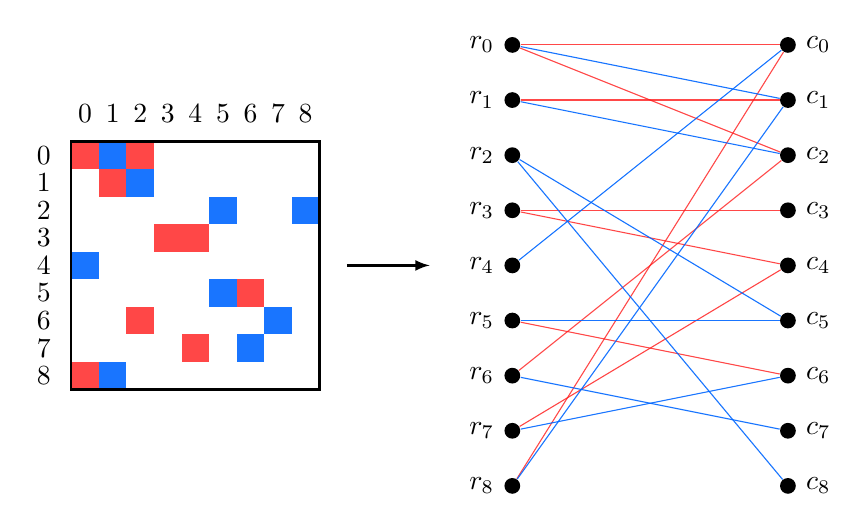
\begin{tikzpicture}[scale=0.35]
		\foreach \x / \y in {1/1,1/3,2/2,4/5,4/4,7/3,8/5,6/7,9/1} { \fill[myred] ({\y-1},{-\x+1}) rectangle +(1,-1);}
		\foreach \x / \y in {1/2,2/3,3/6,3/9,6/6,5/1,7/8,8/7,9/2} { \fill[myblue] ({\y-1},{-\x+1}) rectangle +(1,-1);}
%		\draw[semithick] (0,-9) grid (9,0);
		\draw[thick] (0,-9) rectangle (9,0);

		\draw[myarrow,thick] (10,-4.5) -- (13,-4.5);

		\foreach \x in {0,...,8} { 
			\node[vertex,label=left:\(r_{\x}\)] (r\x) at (16,{3.5-2*\x}) {}; 
			\node[vertex,label=right:\(c_{\x}\)] (c\x) at (26,{3.5-2*\x}) {};
			\node at (-1,{-\x-0.5}) {\x};
			\node at (\x+0.5,1) {\x};
		}

		\foreach \x / \y in {0/0,0/2,1/1,3/4,3/3,6/2,7/4,5/6,8/0} { \draw[myred] (r\x) -- (c\y);}
		\foreach \x / \y in {0/1,1/2,2/5,2/8,5/5,4/0,6/7,7/6,8/1} { \draw[myblue] (r\x) -- (c\y);} 
	\end{tikzpicture}
\end{figure}

\end{frame}

\begin{frame}{Maximum independent set}
 \begin{definition}
		An \emph{independent set} is a subset $V' \subseteq V$ such that $ \forall u,v \in V'$, $(u,v) \notin E$.
	A \emph{maximum} independent set is an independent set of $G$ with maximum cardinality. 
 \end{definition}

\begin{itemize}\itemsep=0.3cm
	\item Our desired object is the maximum independent set
	\item The complement of a (maximum) independent set is a (minimum) vertex cover
\end{itemize}

\end{frame}

\begin{frame}{Maximum independent set}
	In general, computing a maximum independent set is as hard as partitioning the matrix (both NP-hard problems).

But, luckily, our graph is bipartite:

	\begin{itemize}\itemsep=0.3cm
		\item K\H{o}nig's Theorem: on bipartite graphs, maximum matchings and minimum vertex covers have the same size;
		\item Hopcroft-Karp algorithm: $\mathcal{O}\left(N\sqrt{m+n}\right)$ algorithm to compute a maximum matching on a bipartite graph
	\end{itemize}

In our case it is not very demanding to compute a maximum independent set.

\end{frame}

%\begin{frame}{Hopcroft-Karp algorithm}
%Devised by John Hopcroft and Richard Karp in 1973.
%
%We start with an empty matching and increase its size in every iteration:
%
%\begin{enumerate}
%\item We construct the directed graph $(L \cup R, D)$ from $M$:
%\begin{itemize}
%	\item edges in the matching go from $R$ to $L$
%	\item edges not in the matching go from $L$ to $R$
%\end{itemize}
%\item \textbf{breadth-first search} from unmatched vertices in $L$, which terminates when unmatched vertices in $R$ are reached. 
%
%	$l_M$ is the length of these shortest augmenting paths;
%\item \textbf{depth-first search} from an unmatched vertex in $R$ from the previous step, terminates whenever we reach an unmatched vertex in $L$, the path found is augmenting. 
%	
%We resume with the next depth-first search from another unmatched vertex in $R$.
%\end{enumerate}
%\end{frame}
%
%\begin{frame}{Hopcroft-Karp algorithm}
%\begin{itemize}\itemsep=0.4cm
%		\item For practical purposes, the minimum vertex cover is constructed along the matching;
%		\item the matching is augmented over several paths simultaneously ($\sqrt{m+n}$ factor in running time);
%		\item the actual running time is usually better than the theoretical one: our matrices are sparse and the graphs is sparse as well, which means fast search phases.
%	\end{itemize}
%\end{frame}

\begin{frame}{Maximum independent set}

	Given the set of indices $I$, let $S_I$ denote the maximum independent set computed on the matrix $A(I)$.

	One partition-oblivious heuristic to compute $v$: 

	\begin{enumerate}
		\item let $I = \{0,\dots,m+n-1\}$, then $v := (S_I,I \setminus S_I)$
	\end{enumerate}


	For partition-aware heuristics, let $U$ be the set of uncut indices, $C$ be the set of cut indices; we have three possibilities:

\begin{enumerate}\itemsep=0.3cm
	\item we compute $S_U$ and have $v := (S_U,U \setminus S_U, C)$;
	\item we compute $S_U$, $S_C$ and have $v := (S_U, U \setminus S_U, S_C, C \setminus S_C)$;
	\item we compute $S_U$, then we define $U' := U \setminus S_U$ and compute $S_{C \cup U'}$, having $v:= (S_U, S_{C \cup U'}, (C \cup U') \setminus S_{C \cup U'})$.
	\end{enumerate}
\end{frame}


\section{Numerical experiments}

\begin{frame}{General framework for experiments}
	\begin{algorithm}[H]
		\small
		\begin{algorithmic}
			\Require{Sparse matrix $A$}
			\Ensure{Partitioning for the matrix $A$}
			\State Partition $A$ with Mondriaan using the default options and the medium-grain method
			\For{$i=1,\dots,iter_{max}$}
			\State Use any of the heuristics described previously to compute $A_r$ and $A_c$
			\State construct $B$ from $A_r$ and $A_c$
			\State Partition $B$ with Mondriaan using the default options and the row-net model
			\State Re-construct $A$ with the new partitioning
			\EndFor
		\end{algorithmic}
	\end{algorithm}

	Unique framework for both partition-oblivious and partition-aware types of heuristics.

\end{frame}

\begin{frame}{Implementation}

	All of the heuristics have been implemented following these steps:

	\begin{enumerate}
		\item MATLAB prototyping
		\item Core C implementation (MATLAB compatibility through MEX files)
		\item Full C implementation
	\end{enumerate}

	The Hopcroft-Karp algorithm for the maximum indipendent set computation was implemented in the Python programming language.

\end{frame}

\begin{frame}{Implementation}

	Randomness involved during the computation of $A_r$ and $A_c$ and during the actual partitioning. To obtain meaningful results:

	\begin{itemize}
		\item 20 independent initial partitionings
		\item for each, 5 independent runs of the heuristic and subsequent partitioning ($iter_{max} = 1$)
	\end{itemize}

	18 matrices used for tests: 
	\begin{itemize}
		\item rectangular vs. square
		\item $10^{th}$ Dimacs Implementation Challenge
	\end{itemize}
\end{frame}

\begin{frame}{Preliminary selection}
	Wide selections of heuristics, preliminary selection is necessary.

	5 matrices used: 

	\begin{itemize}
		\item \texttt{dfl001};
		\item \texttt{tbdlinux};
		\item \texttt{nug30};
		\item \texttt{rgg\_n\_2\_18\_s0};
		\item  \texttt{bcsstk30}. 
	\end{itemize}

\end{frame}

\begin{frame}{Preliminary selection}

	Partition-oblivious heuristics (17 different algorithms):

	\begin{itemize}
		\item In general, results are much worse than medium-grain method.
		\item Mixing rows and columns in partial assignment is a bad idea
		\item Individual assignment of nonzero best strategy (7\% worse than medium-grain)
		\item Maximum independent set computation yields interesting results (16\% lower communication volume in one matrix, but in general 12\% worse than medium-grain)
	\end{itemize}

	2 heuristics (\texttt{po\_localview} and \texttt{po\_is}) selected for deeper investigation.

\end{frame}

\begin{frame}{Preliminary selection}

	Partition-aware heuristics (21 different algorithms):

	\begin{itemize}
		\item Results closer to medium-grain efficiency
		\item SBD and SBD2 forms are not wortwhile, nor individual assignment of nonzeros
		\item Mixing rows and columns is still not a good idea, but less damaging
		\item Refinement in sorting does not yield a substantial difference
		\item Unsorted concatenation of rows and columns produces good results with rectangular matrices: they can be combined into a \texttt{localbest} heuristic
		\item Maximum independent set strategy very close to medium-grain, even better in a few matrices
	\end{itemize}

	5 heuristics (\texttt{pa\_row}, \texttt{pa\_col}, \texttt{pa\_simple}, \texttt{pa\_is\_1}, \texttt{pa\_is\_3}) selected for deeper investigation.

\end{frame}

\begin{frame}{Number of iterations}
	\begin{textblock}{170}(15,40)
		We are developing a fully iterative scheme: how many iterations do we execute?

		We run the 5 partition-aware selected heuristics for 10 consecutive iterations for each matrix

	\end{textblock}

	\only<1-5>{
		\vspace{1.5cm}
		\begin{figure}[h]
			\centering
			\only<1>{\includegraphics[scale=0.4]{../img/iter_dfl.pdf}}
			\only<2>{\includegraphics[scale=0.4]{../img/iter_nug30.pdf}}
			\only<3>{\includegraphics[scale=0.4]{../img/iter_bcs.pdf}}
			\only<4>{\includegraphics[scale=0.4]{../img/iter_tbdlinux.pdf}}
			\only<5>{\includegraphics[scale=0.4]{../img/iter_delaunay.pdf}}
		\end{figure}
	}
	\only<6>{
	\begin{itemize}\itemsep=0.4cm
			\item Usually 1 iteration is enough to show improvements, if any.
			\item More iterations can worsen the communication volume.
		\end{itemize}
	}
\end{frame}

\begin{frame}{Analysis of the performance of the best heuristics}

	Partition-oblivious heuristics:

\begin{itemize}\itemsep=0.4cm
		\item No devised heuristic was able to improve medium-grain
		\item The preliminary results confirmed:

		\begin{itemize}\itemsep=0.3cm
				\item Individual assignment of nonzeros 7\% worse than medium-grain
				\item Computing the maximum independent set 22\% worse than medium-grain
			\end{itemize}
	\end{itemize}
\end{frame}

\begin{frame}{Analysis of the performance of the best heuristics}
	Partition-aware heuristics:

	\begin{itemize}
		\item Results similar to preliminary selections: preliminary matrices were good representatives
		\item Concatenation interesting strategy:
			\begin{itemize}
				\item \texttt{pa\_row} and \texttt{pa\_col} 8\% worse than medium-grain
				\item \texttt{localbest} method takes best of both: only 4\% worse than medium-grain 
			\end{itemize}
		\item Similar good results for the other strategies (between 4\% and 8\% higher communication volume than medium-grain)
		\item No algorithm was able to beat medium-grain
		\item Considering only rectangular matrices, our methods work better: they improve medium-grain, even if only by little (1-2\%)
	\end{itemize}
\end{frame}

\begin{frame}{Iterative refinement}
	Is there something we can do to improve the results?

	Medium-grain employs a procedure of \textbf{iterative refinement}:

	\begin{enumerate}
		\item $A$ is partitioned into two sets ($A_0$ and $A_1$)
		\item we create again the matrix $B$ of the medium-grain method (example: $A_r = A_0$ and $A_c = A_1$)
		\item we retain communication volume: the first $n$ columns of $B$ are assigned to a single processor, and similarly for the other $m$
		\item we create the hypergraph from this $B$ and a single run of Kernighan-Lin is performed
		\item we repeat steps 1-4 until no improvement is found, then we swap the roles of $A_0$ and $A_1$ for the creation of $A_r$ and $A_c$
		\item we repeat step 5 until no other improvement is found
	\end{enumerate}

\end{frame}

\begin{frame}{Iterative refinement}
	Kernighan-Lin method is \textbf{monotonically non-increasing}: during iterative refinement, the communication volume is either lowered or remains at the same value.

Example of the construction of $B$:
\begin{figure}[h]
	\begin{tikzpicture}[scale=0.2]%,font=\large]
	\only<1->{	
		\foreach \x / \y in {1/1,1/3,2/2,4/5,4/4,3/11,4/9,6/7,1/10,2/7} { \fill[myred] ({\y-1},{-\x+1}) rectangle +(1,-1);}
		\foreach \x / \y in {1/2,2/3,3/6,3/9,6/6,5/1,5/12,6/10,2/11,2/8} { \fill[myblue] ({\y-1},{-\x+1}) rectangle +(1,-1);}
		\draw[thick] (0,-6) rectangle (12,0);
		\node at (6,-7) {$A$};
	}
		\visible<2->{
		\foreach \x / \y in {1/1,1/3,2/2,4/5,4/4,3/11,4/9,6/7,1/10,2/7}{ \fill[purple!90,opacity=.8] ({18+\y-1},{-6-\x+1}) rectangle +(1,-1);}
		\node at (24,-13) {$A_c$};
		\draw[thick] (18,{-6-6}) rectangle ({18+12},-6);

		\foreach \x / \y in  {1/2,2/3,3/6,3/9,6/6,5/1,5/12,6/10,2/11,2/8} { \fill[yellow!60!cyan,opacity=.9] ({18+\y-1},{6-\x+1}) rectangle +(1,-1);}
		\node at (24,-1) {$A_r$};
		\draw[thick] (18,{-6+6}) rectangle ({18+12},6);
		\draw[line width=1.3pt,>=latex,->] (13,-3) -- (17,-9);
		\draw[line width=1.3pt,>=latex,->] (13,-3) -- (17,3);
	}
\visible<3->{
	\only<-3>{
	\foreach \x / \y in {1/1,1/3,2/2,4/5,4/4,3/11,4/9,6/7,1/10,2/7}{ \fill[purple!90,opacity=.8] ({36+\y-1},{-6-\x+1}) rectangle +(1,-1);}
	\foreach \x / \y in  {1/2,2/3,3/6,3/9,6/6,5/1,5/12,6/10,2/11,2/8} { \fill[yellow!60!cyan,opacity=.9] ({48+\x-1},{6-\y+1}) rectangle +(1,-1);}
	\draw[line width=1.3pt,>=latex,->] (31,-9) -- (35,-4);
		\draw[line width=1.3pt,>=latex,->] (31,3) -- (35,-2);


		\foreach \x in {1,2,3,9,10,11} { \fill[gray!10!black,opacity=.9] ({36+\x-1},{6-\x+1}) rectangle +(1,-1);}
		\foreach \x in {1,2,3,6} { \fill[gray!10!black,opacity=.9] ({48+\x-1},{-6-\x+1}) rectangle +(1,-1);}

		\draw[thick] (36,-12) rectangle (54,6);
		\draw[ultra thick] (48,-12) -- (48,6);
		\draw[ultra thick] (36,-6) -- (54,-6);

		\node at (45,-13) {$B$};
	}\only<4->{
	\foreach \x / \y in {1/1,1/3,2/2,4/5,4/4,3/11,4/9,6/7,1/10,2/7}{ \fill[myred] ({36+\y-1},{-6-\x+1}) rectangle +(1,-1);}
	\foreach \x / \y in  {1/2,2/3,3/6,3/9,6/6,5/1,5/12,6/10,2/11,2/8} { \fill[myblue] ({48+\x-1},{6-\y+1}) rectangle +(1,-1);}
	\draw[line width=1.3pt,>=latex,->] (31,-9) -- (35,-4);
		\draw[line width=1.3pt,>=latex,->] (31,3) -- (35,-2);


		\foreach \x in {1,2,3,9,10,11} { \fill[myred] ({36+\x-1},{6-\x+1}) rectangle +(1,-1);}
		\foreach \x in {1,2,3,6} { \fill[myblue] ({48+\x-1},{-6-\x+1}) rectangle +(1,-1);}

		\draw[thick] (36,-12) rectangle (54,6);
		\draw[ultra thick] (48,-12) -- (48,6);
		\draw[ultra thick] (36,-6) -- (54,-6);

		\node at (45,-13) {$B$};
	}
	}
		
	\end{tikzpicture}
\end{figure}
\end{frame}

\begin{frame}{Iterative refinement}
	With iterative refinements, results are in general better:

	\begin{itemize}
		\item partition-oblivious algorithms:
			\begin{itemize}
				\item \texttt{po\_localview} still 7\% worse than medium-grain
				\item \texttt{po\_is} now 6\% worse than medium-grain (down from 22\%)
			\end{itemize}
		\item partition-aware algorithms:
			\begin{itemize}
				\item \texttt{pa\_row} and \texttt{pa\_col} now 2\% and 1\% worse than medium-grain (down from 8\%)
				\item \texttt{localbest} now 1\% \textbf{better} than medium-grain (down from 4\% worse)
				\item \texttt{pa\_simple} now 2\% worse than medium-grain (down from 4\%)
				\item \texttt{pa\_is\_1} and \texttt{pa\_is\_3} now 1\% worse than medium-grain (down from 5\% and 8\%)
			\end{itemize}
	\end{itemize}

	Now, with rectangular matrices, computing the independent set produces an average communication volume 4\% lower than medium-grain.

\end{frame}


\section{Conclusions}

\begin{frame}{Conclusions}
	We originally had two research directions:

\begin{itemize}\itemsep=0.5cm
		\item Improving the quality of the initial partitioning
		\visible<2>{	\begin{itemize}\itemsep=0.4cm
		\item We were not able to outperform medium-grain
	\end{itemize}}
 		\item Developing a fully-iterative scheme
		\visible<3>{			\begin{itemize}\itemsep=0.4cm
				\item We were able to outperform medium-grain only by a small margin
		\item Computing the independent set is worthwile. Also results about concatenation of rows and columns can be explained with it.
		\item Our approach works well with rectangular matrices
	\end{itemize}}
	\end{itemize}
\end{frame}

\begin{frame}{Further research}

A number of possibilities for further development:

\begin{itemize}
	\item Keep testing other strategies to gain more confidence on medium-grain
	\item Hopcroft-Karp algorithm could be implemented in C to tackle bigger problems
	\item Maximum weighted independent match to maximize the number of nonzero completely assigned
	\item If our approach is confirmed to work consistently well with rectangular matrices, it could be added to Mondriaan:
		\begin{enumerate}
			\item The program detects that the matrix is strongly rectangular and asks user for input
			\item The user decides whether he wants to sacrifice computation time for a better partitioning
			\item If so, our approach is executed.
		\end{enumerate}
\end{itemize}
	
\end{frame}
\end{document} 
